\documentclass[a4paper,12pt]{article}
\usepackage[utf8]{inputenc}
\usepackage[T1]{fontenc}
\usepackage{geometry}
\usepackage{graphicx}
\usepackage{subcaption}
\usepackage{booktabs}
\usepackage{amsmath}
\usepackage{hyperref}
\usepackage{tocloft}
\usepackage{setspace}
\usepackage{float}
\usepackage{cite}

\usepackage{tikz}
\usetikzlibrary{arrows.meta, positioning}
\tikzset{
	gene/.style={circle, draw, minimum size=8mm, font=\sffamily},
	activate/.style={-{Stealth[length=3mm]}, thick},
	activate dashed/.style={-{Stealth[length=3mm]}, thick, dashed},
	suppress/.style={-|, thick}
}


\geometry{margin=1in}
\onehalfspacing


\renewcommand{\cftsecleader}{\cftdotfill{\cftdotsep}}

\title{Project Report: [Dynamical analyze of GRN for AML]}
\author{[ Yasaman Safayi Konjin \\ Spehr Salmani Yeganeh \\ Sara Akbari Khorram] \\ [physics , sharif university of technology] \\ [Your Email(s)]}
\date{September 2025}




\begin{document}

\begin{titlepage}
	\centering
	{\large Sharif University of Technology\par}
	\begin{figure}
		\centering
		\includegraphics[width=0.5\linewidth]{csm_kisspng-sharif-university-of-technology-university-of-teheran_7c97300984.png}
		\label{fig:placeholder}
	\end{figure}
	{\large Physics Department \\ Special Topics in Statistical Physics \par}
	\vspace{1 cm}
	{\Huge \bfseries Dynamical Analyze of GRN for AML \par}
	\vspace{1cm}
	{\Large Yasaman Safayi Konjin \\ Sepehr Salmani Yeganeh \\ Sara Akbari Khorram \par}
	\vspace{1 cm}
	
	{\large spring of 2025 \par}
\end{titlepage}

\clearpage

\tableofcontents
\clearpage


%%%%%%%%%%%%%%%%%%%%%%%%%%%%%%%%%%%%%%%%%%%%%%%%%%%%%%%%%%%%%%%%%%%%%%%%%%%
%%%%%%%%%%%%%%%%%%%%%%%%%%%%%%%%%%%%%%%%%%%%%%%%%%%%%%%%%%%%%%%%%%%%%%%%%%%
\section*{Abstract}
\addcontentsline{toc}{section}{Abstract}
This report presents the outcomes of a collaborative project focused on analyzing the dynamics of the gene regulatory network (GRN) associated with acute myeloid leukemia (AML). The primary objective was to develop a computational model to reconstruct AML’s GRN, enabling the study of the disease through the activities of its most influential transcription factors.
Initially, comprehensive data on AML were collected from relevant literature to inform the modeling process. The innovative aspect of this project lies in analyzing network dynamics using a physics-based approach—specifically, leveraging the Jacobian matrix, a method not previously applied in this context.
A Python-based model was developed to generate a dataset capturing potential irregular dynamics that may contribute to cancer development. This dataset was analyzed using the k-means clustering method to identify patterns in transcription factor activity. The results demonstrated a promising alignment with documented transcription factor behaviors in AML cases reported in the literature.
Furthermore, a Random Forest machine learning algorithm was employed to detect irregularities in transcription factor activities and diagnose underlying dynamics. These findings offer valuable insights into AML’s genetic dynamics and pave the way for future research in targeted diagnostics and therapeutic strategies.


%%%%%%%%%%%%%%%%%%%%%%%%%%%%%%%%%%%%%%%%%%%%%%%%%%%%%%%%%%%%%%%%%%%%%%%%%%%
%%%%%%%%%%%%%%%%%%%%%%%%%%%%%%%%%%%%%%%%%%%%%%%%%%%%%%%%%%%%%%%%%%%%%%%%%%%
\section{Introduction}
\subsection{Problem Statement}
\textit{Acute Myeloid Leukemia} (AML) is a complex hematologic malignancy characterized by dysregulated gene expression, driven by aberrant dynamics in its \textit{gene regulatory network} (GRN). Despite advances in understanding AML’s molecular basis, current computational models often fail to capture the intricate dynamics of transcription factor interactions that drive disease progression. Traditional approaches to GRN analysis—such as differential expression studies—lack the capacity to model the nonlinear and dynamic behavior of gene interactions, limiting their effectiveness in identifying critical regulatory patterns.

Moreover, there remains a gap in applying physics-based methodologies, such as Jacobian matrix analysis, to the study of AML’s GRN - an approach that could uncover novel insights into its genetic dynamics. This project addresses the need for an innovative computational framework to reconstruct and analyze AML’s GRN, with a focus on identifying irregular transcription factor activities. By leveraging a physics-based approach, this study aims to deepen our understanding of AML’s regulatory mechanisms and support the development of targeted diagnostic and therapeutic strategies.

%%%%%%%%%%%%%%%%%%%%%%%%%%%%%%%%%%%%%%%%%%%%%%%%%%%%%%%%%%%%%%%%%%%%%%%%%%%
\subsection{Objectives}
The objectives of this project are as follows:
\begin{enumerate}
	\item To develop a computational model for reconstructing the gene regulatory network (GRN) of acute myeloid leukemia (AML) using a physics-based approach that leverages the Jacobian matrix.
	\item To generate a dataset that captures irregular dynamics in transcription factor activities potentially contributing to AML progression.
	\item To analyze the generated dataset using the k-means clustering method in order to identify patterns in transcription factor behavior.
	\item To implement a Random Forest machine learning algorithm for detecting and diagnosing irregularities in transcription factor activities within the AML GRN.
	\item To validate the model’s findings against existing literature, assessing its accuracy and potential to advance targeted diagnostic and therapeutic strategies.
\end{enumerate}



%%%%%%%%%%%%%%%%%%%%%%%%%%%%%%%%%%%%%%%%%%%%%%%%%%%%%%%%%%%%%%%%%%%%%%%%%%%
%%%%%%%%%%%%%%%%%%%%%%%%%%%%%%%%%%%%%%%%%%%%%%%%%%%%%%%%%%%%%%%%%%%%%%%%%%%
\section{Methodology}
This section describes the computational methods employed to reconstruct and analyze the gene regulatory network (GRN) of acute myeloid leukemia (AML), with a particular focus on the dynamics of six key transcription factors: \textit{CEBPA}, \textit{SPI1}, \textit{MYB}, \textit{RUNX1}, \textit{HOXA9}, and \textit{MEIS1}. The GRN illustrated in Figure~\ref{fig:gene_network} represents the hypothetical framework adopted for the subsequent analyses \cite{Maura2021,Estey2012,Storrie2016,Grimwade1995,Papaemmanuil2016,Ley2013}.


\begin{figure}[tp]
	\centering
	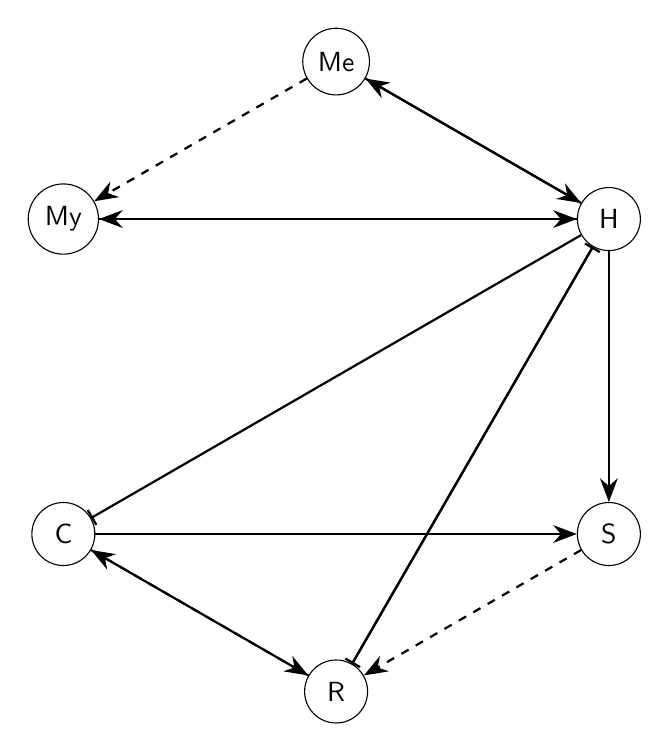
\begin{tikzpicture}[node distance=2cm]
		
		% Place nodes in a circle
		\node[gene] (Me) at (90:4cm) {Me};
		\node[gene] (H)  at (30:4cm) {H};
		\node[gene] (S)  at (-30:4cm) {S};
		\node[gene] (R)  at (-90:4cm) {R};
		\node[gene] (C)  at (-150:4cm) {C};
		\node[gene] (My) at (150:4cm) {My};
		
		% Edges
		\draw[activate dashed] (Me) -- (My);   % Me -> My (dashed)
		\draw[activate] (Me) -- (H);            % Me -> H (solid)
		
		\draw[activate dashed] (My) -- (H);     % My -> H (dashed)
		
		\draw[activate] (H) -- (My);            % H -> My (solid)
		\draw[activate] (H) -- (Me);            % H -> Me (solid)
		\draw[suppress] (H) -- (R);             % H -| R
		\draw[suppress] (H) -- (C);             % H -| C
		\draw[activate] (H) -- (S);             % H -> S
		
		\draw[activate] (C) -- (S);             % C -> S
		\draw[activate dashed] (C) -- (R);      % C -> R (dashed)
		
		\draw[activate dashed] (S) -- (R);      % S -> R (dashed)
		
		\draw[activate] (R) -- (C);             % R -> C
		\draw[suppress] (R) -- (H);             % R -| H
		
	\end{tikzpicture}
	\caption{Gene regulatory network showing activation (solid/dashed arrows) and suppression (flat-head lines) among Me, My, H, R, C, and S.}
	\label{fig:gene_network}
\end{figure}

%%%%%%%%%%%%%%%%%%%%%%%%%%%%%%%%%%%%%%%%%%%%%%%%%%%%%%%%%%%%%%%%%%%%%%%%%%%
\subsection{Data Collection and Parameter Setup}
\label{subsec:data_collection}
A simulated dataset was generated to represent the dynamics of AML’s GRN, focusing on six transcription factors. Interaction parameters were defined as a symbolic matrix \( A \) with 19 parameters (e.g., \( cc \), \( rc \), \( hc \)), representing regulatory interactions. Mean and standard deviation values for scaling fixed points were assigned based on hypothetical RNA-seq data.

%%%%%%%%%%%%%%%%%%%%%%%%%%%%%%%%%%%%%%%%%%%%%%%%%%%%%%%%%%%%%%%%%%%%%%%%%%%
\subsection{Model Development}
\label{subsec:model_development}
A Python-based computational model was developed to reconstruct AML’s GRN using the Jacobian matrix. The matrix \( \mathbf{A} \), representing GRN interactions, was constructed using \texttt{SymPy} for symbolic computations and converted to numerical form with \texttt{NumPy} and \texttt{SciPy}. The condition for non-zero fixed points was derived by solving \( \det(\mathbf{A}) = 0 \) for the parameter \( cc \).

To ensure a robust representation of the GRN and mitigate matrix sparsity, hypothetical regulatory links were incorporated into the symbolic matrix. A total of 42,208 valid parameter sets were generated by randomly sampling 18 parameters within predefined ranges (e.g., \( \texttt{activation constants} \in [0.01, 2] \), \( \texttt{suppression constants} \in [-2, -0.01] \), \( \texttt{self-activation and suppression rate} \in [-2, 2] \), \( \texttt{hypothetical links} \in [0, 1] \)), while ensuring \( \det(\mathbf{A}) \approx 0 \). Fixed points were computed using the null space of \( \mathbf{A} \) and scaled to RNA-seq ranges using predefined means and standard deviations. Data generation continued iteratively until exactly \( \texttt{number\_of\_stable\_fixed\_points} = 512 \) stable fixed points were obtained, ensuring sufficient representation of stable system dynamics for downstream analyses.


%%%%%%%%%%%%%%%%%%%%%%%%%%%%%%%%%%%%%%%%%%%%%%%%%%%%%%%%%%%%%%%%%%%%%%%%%%%
\subsection{Dynamic Analysis}
\label{subsec:dynamic_analysis}
The dynamics of the GRN were analyzed by computing the eigenvalues of the numerical Jacobian matrix \( \mathbf{A} \). The real parts of the eigenvalues were used to classify the system’s behavior into Stable, Unstable, Saddle, or Non-zero Fixed Point dynamics, with a threshold of \( \pm 0.0001 \). 

%%%%%%%%%%%%%%%%%%%%%%%%%%%%%%%%%%%%%%%%%%%%%%%%%%%%%%%%%%%%%%%%%%%%%%%%%%%
\subsection{Clustering Analysis}
\label{subsec:clustering}
The fixed points dataset, comprising expression levels of the six transcription factors, was normalized using \texttt{StandardScaler} from \texttt{scikit-learn}. The k-means clustering algorithm was applied to identify patterns in transcription factor dynamics, with the optimal number of clusters determined using the silhouette score over a range of \( k = 2 \) to \( 9 \). Clustering results were visualized in 2D and 3D using UMAP (\texttt{n\_neighbors=30}, \texttt{min\_dist=0.5}) and PCA, implemented with \texttt{umap-learn} and \texttt{scikit-learn} libraries, respectively. Visualizations were generated using \texttt{Matplotlib} and \texttt{Plotly} to analyze cluster distributions.

%%%%%%%%%%%%%%%%%%%%%%%%%%%%%%%%%%%%%%%%%%%%%%%%%%%%%%%%%%%%%%%%%%%%%%%%%%%
\subsection{Diagnostic Modeling with Random Forest}
\label{subsec:diagnostic_modeling}
A Random Forest classifier, implemented via \texttt{scikit-learn}, was trained to classify GRN dynamics (Stable, Unstable, Saddle, Non-zero Fixed Points) based on the dataset of fixed points and interaction parameters. Two sampling strategies were employed to construct training datasets. The first, referred to as \texttt{custom\_sampling}, included all stable and non-zero fixed points along with a fraction of saddle points proportional to the size of the other classes. The second, referred to as \texttt{undersampling}, selected an equal number of samples from each class to balance the dataset. 

The model was evaluated in two ways: (i) using a train-test split (80\% training, 20\% testing) on the sampled datasets, and (ii) applying the same split to the entire dataset. Features were normalized using \texttt{StandardScaler}, and the model was trained on the scaled training data. Model performance was assessed using accuracy, precision, recall, and F1-score metrics, as reported in a classification report.


%%%%%%%%%%%%%%%%%%%%%%%%%%%%%%%%%%%%%%%%%%%%%%%%%%%%%%%%%%%%%%%%%%%%%%%%%%%
\subsection{Validation}
\label{subsec:validation}
The clustering and classification results were validated by analyzing the distribution of dynamics within each cluster and computing statistical measures, such as the mean and standard deviation of fixed points and interaction parameters. The silhouette score assessed clustering quality, while the Random Forest model’s classification report ensured robust detection of dynamics. Findings were compared with documented AML transcription factor behaviors to evaluate their biological relevance.


%%%%%%%%%%%%%%%%%%%%%%%%%%%%%%%%%%%%%%%%%%%%%%%%%%%%%%%%%%%%%%%%%%%%%%%%%%%
%%%%%%%%%%%%%%%%%%%%%%%%%%%%%%%%%%%%%%%%%%%%%%%%%%%%%%%%%%%%%%%%%%%%%%%%%%%
\section{Results}
\label{sec:results}
The results are very promising. We identified parameter sets that resulted in stable fixed points, indicating that a GRN with these parameters could plausibly exist in the real world. Clustering on the fixed points revealed distinct dynamic patterns that, when compared with real data, could be used to infer different biological states and distinguish healthy samples from cancerous ones. Furthermore, the Random Forest model demonstrated its potential to aid in the diagnosis of AML using patient RNA-seq data.

%%%%%%%%%%%%%%%%%%%%%%%%%%%%%%%%%%%%%%%%%%%%%%%%%%%%%%%%%%%%%%%%%%%%%%%%%%%
\subsection{Clustering All Fixed Points}
All fixed points obtained from the parameter sets were successfully clustered into nine well-separated groups. The separation of these clusters is most clearly observed in the three-dimensional visualizations, which can be reproduced by running the provided code. These clusters capture distinct dynamic behaviors arising from different configurations of the interaction matrix \( \mathbf{A} \), thereby enabling us to distinguish between the various dynamical regimes of the GRN.

Representative visualizations of the clustering results using PCA and UMAP are shown in Figure~\ref{fig:all-fixed-points}. Detailed numerical results, including cluster assignments and statistical summaries, are provided in the file \texttt{stat-cluster.txt} available in the project’s GitHub repository.

\begin{figure}[H]
\centering
\begin{subfigure}{0.45\textwidth}
	\includegraphics[width=\textwidth,height=\textwidth]{PCA-2D}
	\caption{}
\end{subfigure}
\hfill
\begin{subfigure}{0.45\textwidth}
	\includegraphics[width=\textwidth,height=\textwidth]{PCA-3D}
	\caption{}
\end{subfigure}
\hfill
\begin{subfigure}{0.45\textwidth}
	\includegraphics[width=\textwidth,height=\textwidth]{UMAP-2D}
	\caption{}
\end{subfigure}
\hfill
\begin{subfigure}{0.45\textwidth}
	\includegraphics[width=\textwidth,height=\textwidth]{UMAP-3D}
	\caption{}
\end{subfigure}
\caption{Clusters of all fixed points visualized by PCA in (a) two and (b) three dimensions, and by UMAP in (c) two and (d) three dimensions.}
\label{fig:all-fixed-points}
\end{figure}

%%%%%%%%%%%%%%%%%%%%%%%%%%%%%%%%%%%%%%%%%%%%%%%%%%%%%%%%%%%%%%%%%%%%%%%%%%%
\subsection{Clustering Stable Fixed Points}
In this analysis, clustering was performed exclusively on the subset of stable fixed points, resulting in three distinct clusters (Figure~\ref{fig:stable-fixed-points}). Within these clusters, fixed points exhibiting extreme expression levels-where at least one gene was expressed significantly above or below expected RNA-seq ranges-were marked as indicative of cancerous states.

This separation highlights the model’s ability to distinguish between healthy and cancer-like dynamics based solely on GRN parameters. The emergence of cancer-associated fixed points from specific parameter configurations suggests that the model can simulate how variations in GRN structure may lead to pathological behavior, offering insight into the mechanistic origins of AML.

Detailed clustering results, including statistical summaries and cluster assignments, are available in the file \texttt{stat-cluster-stable.txt} on the project’s GitHub repository. For enhanced interpretation, users are encouraged to view the three-dimensional plots generated by the code, which provide clearer visual separation between clusters.

\begin{figure}[tp]
\centering
\begin{subfigure}{0.45\textwidth}
	\includegraphics[width=\textwidth,height=\textwidth]{stable-PCA-2D-flagged}
	\caption{}
\end{subfigure}
\hfill
\begin{subfigure}{0.45\textwidth}
	\includegraphics[width=\textwidth,height=\textwidth]{stable-PCA-3D-flagged}
	\caption{}
\end{subfigure}
\hfill
\begin{subfigure}{0.45\textwidth}
	\includegraphics[width=\textwidth,height=\textwidth]{stable-UMAP-2D-flagged}
	\caption{}
\end{subfigure}
\hfill
\begin{subfigure}{0.45\textwidth}
	\includegraphics[width=\textwidth,height=\textwidth]{stable-UMAP-3D-flagged}
	\caption{}
\end{subfigure}
\caption{Clusters of stable fixed points visualized with PCA in (a) two and (b) three dimensions, and with UMAP in (c) two and (d) three dimensions. Cancerous points are highlighted with an ``x'' to distinguish them from healthy ones.}
\label{fig:stable-fixed-points}
\end{figure}

%%%%%%%%%%%%%%%%%%%%%%%%%%%%%%%%%%%%%%%%%%%%%%%%%%%%%%%%%%%%%%%%%%%%%%%%%%%
\subsection{Classification of GRN Dynamics with Random Forest}
To evaluate the predictive power of our framework, a Random Forest classifier was trained to categorize GRN dynamics into four classes: Stable, Unstable, Saddle, and Non-zero Fixed Points. Both unbiased sampling strategies were applied, and in each case the model achieved strong performance. 

Using the \texttt{custom\_sampling} approach, which included all stable and non-zero fixed points together with a proportional subset of saddle points, the classifier reached an accuracy of approximately 96\% in correctly identifying the dynamic type. The \texttt{undersampling} strategy, which balanced the dataset by selecting an equal number of samples from each class, yielded a very similar result with an accuracy of about 96\%. 

These results demonstrate the robustness of the Random Forest model across different sampling schemes and highlight its potential applicability to real-world data. In particular, they suggest that when applied to patient RNA-seq profiles, the model could serve as a diagnostic tool for distinguishing healthy from AML-associated regulatory dynamics. Complete details of the classification results are provided in the files \texttt{stat-learn-custom.txt} and \texttt{stat-learn-under.txt} available in the project’s GitHub repository.


%%%%%%%%%%%%%%%%%%%%%%%%%%%%%%%%%%%%%%%%%%%%%%%%%%%%%%%%%%%%%%%%%%%%%%%%%%%
%%%%%%%%%%%%%%%%%%%%%%%%%%%%%%%%%%%%%%%%%%%%%%%%%%%%%%%%%%%%%%%%%%%%%%%%%%%
\section{Discussion}
The findings of this study demonstrate the effectiveness of combining physics-based modeling with machine learning to analyze the dynamics of the gene regulatory network (GRN) associated with acute myeloid leukemia (AML). By leveraging Jacobian matrix analysis, we were able to generate parameter sets that produced stable fixed points, providing a plausible representation of biologically meaningful states. The clustering of these fixed points revealed distinct dynamical regimes, with certain clusters corresponding to cancer-like states characterized by extreme transcription factor expression. This highlights the model’s ability to capture both healthy and pathological behaviors within the same computational framework.

The clustering results underscore the interpretability of GRN dynamics: nine clusters were identified when considering all fixed points, while restricting the analysis to stable fixed points yielded three well-separated groups. Importantly, the emergence of cancer-associated fixed points from specific parameter configurations suggests that subtle variations in GRN structure can drive the transition from healthy to malignant states. This provides a mechanistic perspective on how AML may arise from dysregulated transcription factor interactions.

The Random Forest classifier further validated the predictive power of the framework, achieving approximately 96\% accuracy under both custom sampling and undersampling strategies. The consistency of these results across different sampling schemes demonstrates the robustness of the approach. More importantly, it suggests that when applied to real-world patient RNA-seq data, the model could serve as a diagnostic tool capable of distinguishing AML-associated dynamics from healthy regulatory states. This translational potential represents a significant step toward computational diagnostics in hematologic malignancies.

While the present work is based on simulated data, the framework is readily extendable to experimental datasets. Incorporating real patient-derived transcriptomic data would allow for more precise mapping between GRN parameters and biological states, thereby enhancing both diagnostic accuracy and mechanistic insight. Future work will focus on scaling the model to larger networks, integrating additional transcription factors, and validating predictions against clinical datasets. Such extensions could not only improve diagnostic capabilities but also shed light on the pathways through which AML emerges and progresses.


%%%%%%%%%%%%%%%%%%%%%%%%%%%%%%%%%%%%%%%%%%%%%%%%%%%%%%%%%%%%%%%%%%%%%%%%%%%
%%%%%%%%%%%%%%%%%%%%%%%%%%%%%%%%%%%%%%%%%%%%%%%%%%%%%%%%%%%%%%%%%%%%%%%%%%%
\section{Conclusion}
In conclusion, this study establishes a proof of concept for using dynamical systems analysis and machine learning to investigate AML’s gene regulatory network. By bridging mathematical modeling with biological interpretation, we provide a framework that is both computationally rigorous and biologically meaningful. Given real-world data, this approach has the potential to significantly advance our ability to diagnose AML and to uncover the regulatory mechanisms underlying its creation and progression.


%%%%%%%%%%%%%%%%%%%%%%%%%%%%%%%%%%%%%%%%%%%%%%%%%%%%%%%%%%%%%%%%%%%%%%%%%%%
%%%%%%%%%%%%%%%%%%%%%%%%%%%%%%%%%%%%%%%%%%%%%%%%%%%%%%%%%%%%%%%%%%%%%%%%%%%
\section{Code Availability}
The source code developed and used in this study is openly available at the GitHub repository:  
\url{https://github.com/SepehrSYeganeh/Gene-Dynamics}. 
All plots and supplementary files, including those not presented in this manuscript, can be accessed there.


\begin{thebibliography}{99}
	
	\bibitem{Maura2021}
	F. Maura, A. Dodero, C. Carniti, N. Bolli, M. Magni, V. Monti, A. Cabras, D. Leongamornlert, F. Abascal, B. Diamond, B. Rodriguez-Martin, J. Zamora, A. Butler, I. Martincorena, J. M. C. Tubio, P. J. Campbell, A. Chiappella, G. Pruneri, and P. Corradini.  
	\newblock CDKN2A deletion is a frequent event associated with poor outcome in patients with peripheral T-cell lymphoma not otherwise specified (PTCL-NOS).  
	\newblock \textit{Haematologica}, 106(11):2870--2881, 2021.  
	DOI: \href{https://doi.org/10.3324/haematol.2020.262659}{10.3324/haematol.2020.262659}.
	
	\bibitem{Estey2012}
	E. Estey.  
	\newblock Acute myeloid leukemia: 2012 update on risk-stratification and management.  
	\newblock \textit{Blood}, 119(19):4408--4416, 2012.  
	DOI: \href{https://doi.org/10.1182/blood-2012-01-379008}{10.1182/blood-2012-01-379008}.
	
	\bibitem{Storrie2016}
	B. Storrie.  
	\newblock A tip of the cap to procoagulant platelets.  
	\newblock \textit{Blood}, 128(13):1668--1669, 2016.  
	DOI: \href{https://doi.org/10.1182/blood-2016-08-730622}{10.1182/blood-2016-08-730622}.
	
	\bibitem{Grimwade1995}
	D. Grimwade, A. H. Walker, D. Oliver, and others.  
	\newblock The importance of diagnostic cytogenetics on outcome in AML: analysis of 1,612 patients entered into the MRC AML 10 trial.  
	\newblock \textit{Blood}, 86(12):354--365, 1995.  
	DOI: \href{https://doi.org/10.1182/blood.V86.12.354.bloodjournal8612354}{10.1182/blood.V86.12.354.bloodjournal8612354}.
	
	\bibitem{Papaemmanuil2016}
	E. Papaemmanuil, M. Gerstung, L. Bullinger, and others.  
	\newblock Genomic classification and prognosis in acute myeloid leukemia.  
	\newblock \textit{Nature Communications}, 7:11892, 2016.  
	DOI: \href{https://doi.org/10.1038/ncomms11001}{10.1038/ncomms11001}.
	
	\bibitem{Ley2013}
	T. J. Ley, E. R. Mardis, C. A. Miller, and others.  
	\newblock Genomic and epigenomic landscapes of adult de novo acute myeloid leukemia.  
	\newblock \textit{New England Journal of Medicine}, 368(22):2059--2074, 2013.  
	DOI: \href{https://doi.org/10.1056/NEJMoa1301689}{10.1056/NEJMoa1301689}.
	
\end{thebibliography}





\end{document}